%
% Thesis Style 用サンプル TeX
%
% 注意:目次等を作成するために何度か platex にかけること
%
% 両面印刷する時は twoside にする
%
% 12pt にするのは最終手段
%
\documentclass[11pt,oneside,dvipdfmx]{jbook}
\usepackage{csg-thesis}
\usepackage[dvipdfmx]{graphicx}
\usepackage{url}
\usepackage{amsmath}
\usepackage{pdfpages}
\usepackage{float}
\usepackage[a4paper]{geometry}

\usepackage{listings,jvlisting}
\lstset{
  basicstyle={\ttfamily},
  identifierstyle={\small},
  commentstyle={\smallitshape},
  keywordstyle={\small\bfseries},
  ndkeywordstyle={\small},
  stringstyle={\small\ttfamily},
  frame={tb},
  breaklines=true,
  columns=[l]{fullflexible},
  numbers=left,
  xrightmargin=0zw,
  xleftmargin=3zw,
  numberstyle={\scriptsize},
  stepnumber=1,
  numbersep=1zw,
  lineskip=-0.5ex
}

\newcommand{\simname}{[ここにシミュレータの名前を入力]}

\usepackage[dvipdfmx]{hyperref}
\usepackage{pxjahyper}
\hypersetup{%
  setpagesize=false,%
  hidelinks,%
  colorlinks=false,%
  pdftitle={},%
  pdfsubject={},%
  pdfauthor={},%
  pdfkeywords={}%
}

\begin{document}

% 題目
% 適当に\\で区切って見やすくする
\title{%
物理学の学習のためのプログラマブルな
シミュレータと環境の提案
}

% 学位(学部と大学院で変更)
\degree{学士}
%\degree{修士}

% 名前
\author{木内 康介}

% 提出日
\date{令和5年2月6日}

% 卒業年度
\schoolyear{令和4年}

% 所属(学部と大学院で変更)
\department{東京工業大学 情報理工学院 数理・計算科学系}

% 学籍番号
\stnumber{18B04657}

% 指導教員(教官ではなくなった...)
\supervisor{増原 英彦 教授}

\maketitle

%%%%%%%%%%%%%%%%%%%%%%%%%%%%%%%%%%%%%%%%%%%%%%%%%%%%%%%%%%%%%%%%%%%%%%

% 概要
\begin{abstract}
ここにAbstractを書く
\end{abstract}

% 謝辞
\begin{acknowledgments}
本研究を進めるにあたり、増原英彦教授、叢悠悠助教にアドバイスやご指導をいただきました。この場を借りて感謝申し上げます。また、増原研究室の皆様に多くのコメントを頂きました。特に、ご自身の研究でお忙しい中で何度も協力してくださった田辺さん、私と同じく教育に関する研究をしており相談に乗ってくれた角田さん、学生室で雑談相手になってくれた津山くんに深く感謝しております。

% また、 lively.next 開発者の Robin, Linus, Jens にも助けていただきました。
% 本論文は以上の方々のご支援がなければ存在しえませんでした。

\end{acknowledgments}

%%%%%%%%%%%%%%%%%%%%%%%%%%%%%%%%%%%%%%%%%%%%%%%%%%%%%%%%%%%%%%%%%%%%%%

\tableofcontents       %% 目次

%
% 目次等にはローマ数字を使い、本文開始ページを 1 ページ目にできる
% この方が見た目がきれいであるが、全体のページ数は減って見える
% ここでローマ数字に変えた場合は chapter 1 でアラビア数字に戻すこと
%
\pagenumbering{roman}  %% ページ番号をローマ数字にする

% \listoffigures         %% 図目次(図がない場合は不要)
% \listoftables          %% 表目次(表がない場合は不要)

%%%%%%%%%%%%%%%%%%%%%%%%%%%%%%%%%%%%%%%%%%%%%%%%%%%%%%%%%%%%%%%%%%%%%%

\cleardoublepage
\pagenumbering{arabic}  %% ページ番号をローマ数字にする
%
% 本文
%
% 各章を各ファイルに書く
%
\chapter{はじめに} \label{first}
%\pagenumbering{arabic}  %% ページ番号をアラビア数字に変更

高等学校における物理学の授業において、生徒による実験は必要不可欠である。文部科学省が平成30年に告示した高等学校学習指導要領の理科編には以下ように記されている:
\begin{quote}
探究的な学習は教育課程全体を通じて充実を図るべきものであるが,観察・実験等を重視して学習を行う教科である理科がその中核となって探究的な学習の充実を図っていくことが重要である。
\end{quote}
また、[TODO: 実験による学習効果を調査した論文を調べる]

しかし実際は、実験の実施は完全ではない。林らの調査~\cite{2015KJ00010038066}によると、力学分野における最も基本的な「運動の法則」に関する実験の経験は、2014年の調査時点で60\%程度にしか満たない。また、非常によく取り上げられる題材である「モンキーハンティング(\ref{モンキーハンティング})」に関しては10\%に満たない。考えられる理由としては、モンキーハンティングを実験するためには大掛かりな装置と空間が必要になることや、測定が難しいことなどがある。

そこで代替として考えられるのが、シミュレーションの利用である。
% 現在日本ではGIGAスクール構想に基づき、生徒に対して1人1台ずつのコンピュータ端末の配布が進められている。そのため、今まで以上にコンピュータを利用したシミュレーションを活用することが可能である。
簡単に実験ができない内容であったとしても、シミュレーションを用いれば誰でも実験と同様な学習効果を得ることができる。実際 Ajredini~\cite{ajredini_real_2014}は、実際の実験とシミュレーションで得られる知識に大きな差は無いと結論づけている。また、シミュレーションでは実験器具の準備などの作業に割く時間を削減することができ、思考・分析・議論により多くの時間を割くことができるとも述べている。

しかし、既存のシミュレータでは不十分な点も存在する。一般的な物理学の学習用のシミュレータでは、設定されたシチュエーションにおける物体の挙動を観測することはできるが、シチュエーションそのものを大きく変化させることはできない。即ち、「この物体の座標を変更するとどう動くか」「この物体の初速度を変更するとどう動くか」「重力加速度の値を変更するとどう動くか」などといった疑問全てに対するシミュレーションは提供できない。更に、シミュレーションはその特性上数値計算をベースに実行される。一方、大学入試などにおける物理の問題は文字式の計算をベースにしている。そのため、「自分が計算した結果のこの文字式は正しく物理現象を表しているのか」ということを既存のシミュレータで確認することは難しい。

そこで、本論文ではシチュエーションを自分で設定でき、文字式をベースとしたシミュレーションが可能なシミュレータである「\simname」を提案する。

本論文の構成は以下の通りである。
第\ref{related}章で、既存のシミュレータとそれを用いた実例について紹介する。
第\ref{method}章で、\simname の紹介とその効果を説明する。
第\ref{implementation}章で、\simname の実現方法を説明する。
第\ref{evaluation}章で、\simname の評価方法を提案する。
第\ref{conclusion}章で、まとめと今後の展望について述べる。

%%%%
\chapter{関連研究} \label{related}

\section{PhET}

PhET\cite{Perkins2006PhETIS}\cite{PhET}について

PhETを用いた実例
\cite{prima_learning_2018}
\cite{rehman_teaching_2021}

\section{Scratch}

Scratch\cite{Scratch}について

Scratchを用いた実例

\cite{Lpez2015ScratchAA}


%%%%
\chapter{提案する内容}

\begin{itemize}
\item {
  シミュレータの概要
}
\item {
  既存のシミュレータとの差異
}
\end{itemize}

\chapter{実装の方針} \label{implementation}

フロントエンドに lively.next\footnote{\url{https://lively-next.org}} を、方程式の処理と数値計算に SymPy~\cite{meurer_sympy_2017} を用い、JavaScript と Python を組み合わせて実装する。また、 Pyodide~\footnote{\tiny{\url{https://github.com/pyodide/pyodide}}} を用いることで、ブラウザ上で全ての計算を行う。
% lively.next は、GUIアプリケーションを作成・実行するためのWebプログラミング環境である。学習者が物体や方程式を定義する画面とシミュレーションを表示する画面を lively.next で作成する。SymPy は、記号計算のための Python ライブラリであり、Pyodide~\footnote{\tiny{\url{https://github.com/pyodide/pyodide}}} を用いることで WebAssembly に変換し、ブラウザで実行する。\simname は、入力された物理量や方程式を SymPy オブジェクトに変換することで、数値計算を可能にする。シミュレーションの実行時は、設定された時刻 $t$ の範囲を粒度 $\Delta t$ ずつ変化させる。各方程式に各 $t$ を代入した結果を lively.next が受け取り、描画する。シミュレーションのリアルタイム性を確保するため、各 $t$ を方程式に代入した値は方程式の定義時・変数の値の変更時にあらかじめ計算する。

\section{lively.next}
lively.next は Lively~\cite{ingalls_2008}から派生したプロジェクトで、ブラウザ上で GUI アプリケーションを作成・実行することができる Web プログラミング環境である。これを用いて、学習者が物体や方程式を定義する物理系定義ペインと、シミュレーション結果を表示する観測ペインを実装する。ブラウザ上で利用できるため、学習者はソフトウェアのインストールなどをする必要がなく、簡単に利用できる。

\begin{figure}[hbt]
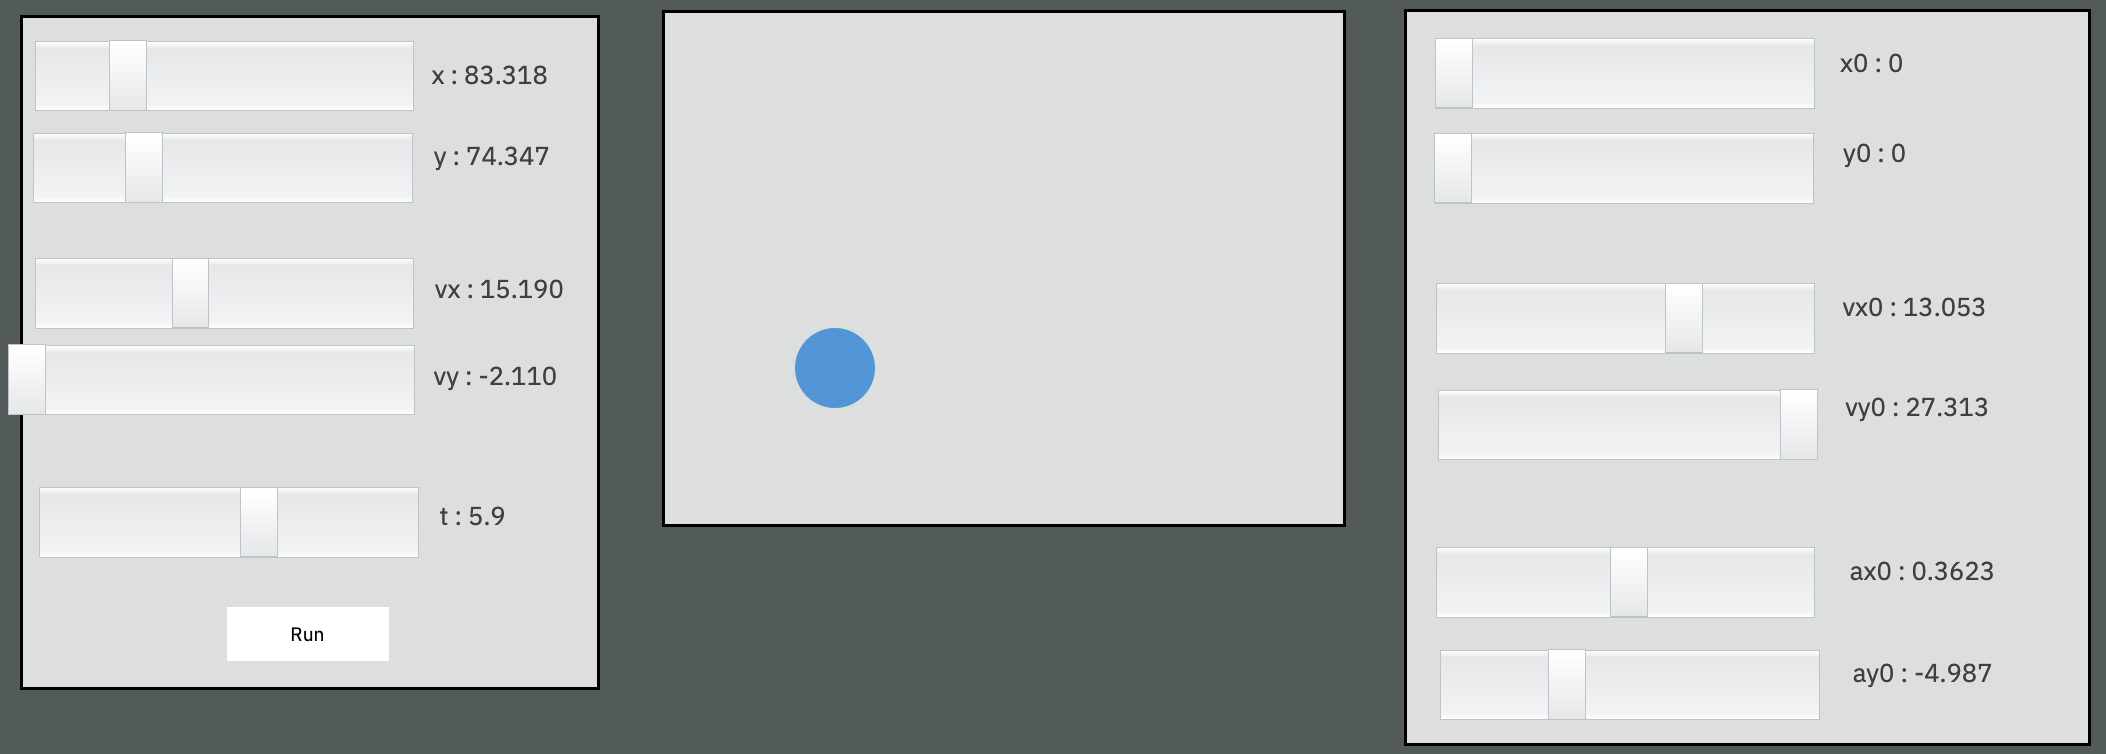
\includegraphics[width=0.9\linewidth]{figure/lively_example.png}
\end{figure}

\section{SymPy}
SymPy は、記号計算のための Python ライブラリである。

% \section{SymPy}
% SymPy は、文字式の計算を可能にするPythonライブラリである。図\ref{SymPy_example}に簡単な例を載せる。SymPyを用いることで、実際に物理の問題を解くように文字式の計算を実行することができる。数値の代入も可能なため、シミュレーションを実行する際は SymPy で表現された式に数値を代入して計算している。

% \clearpage
% \begin{figure}
% 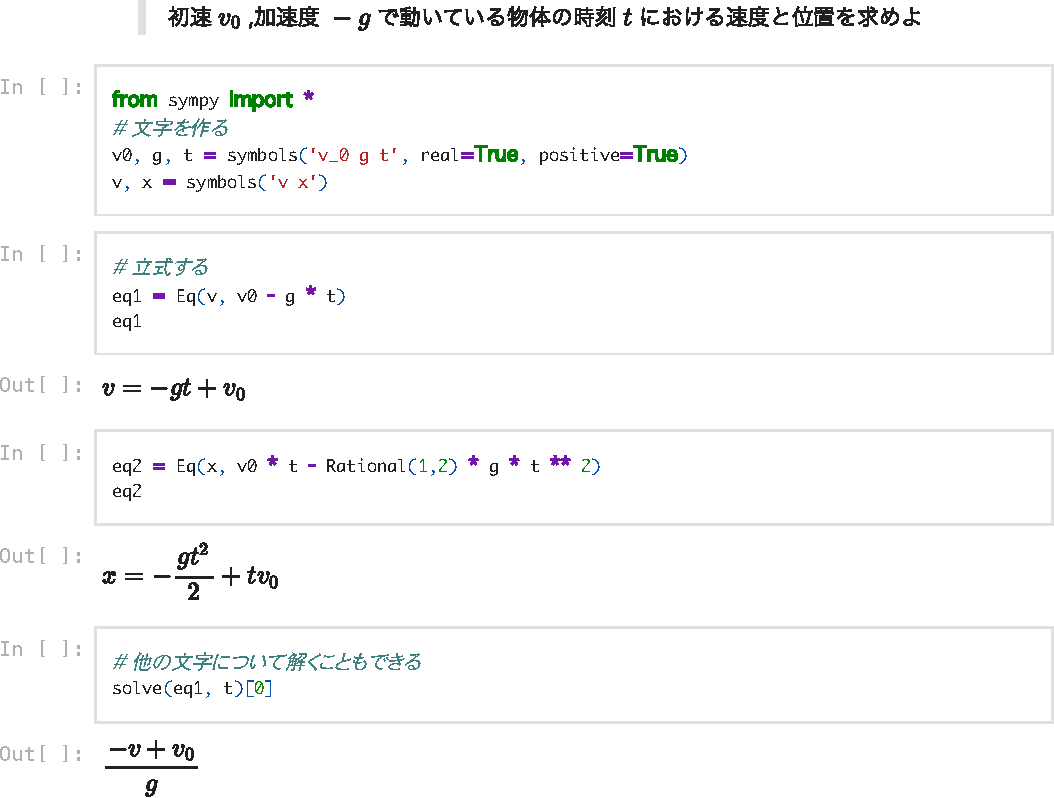
\includegraphics[page=1, scale=.8]{work/SymPy_example-crop.pdf}
% \caption{SymPyを用いた文字式の計算例} \label{SymPy_example}
% \end{figure}
% \clearpage

% \section{Pyodide}
% Pyodide は、Mozilla が開発している WebAssembly で実装された CPython 処理系である。ブラウザ上で Python コードを実行できるほか、メジャーなパッケージにも対応している。 SymPy も Pyodide で実行可能である。実際に Pyodide で SymPy を実行する計算の例を図\ref{Pyodide_example}に、結果を KaTeX を用いて表示した例を図\ref{Pyodide_result}に記す。

% \newgeometry{left=1cm, right=1cm}
% \begin{figure}[htb]
% \begin{lstlisting}[language=html]
% <!DOCTYPE html>
% <head>
%   <script src="https://cdn.jsdelivr.net/pyodide/v0.22.0/full/pyodide.js"></script>
%   <link rel="stylesheet" href="https://cdn.jsdelivr.net/npm/katex@0.16.4/dist/katex.min.css" integrity="sha384-vKruj+a13U8yHIkAyGgK1J3ArTLzrFGBbBc0tDp4ad/EyewESeXE/Iv67Aj8gKZ0" crossorigin="anonymous">
%   <script defer src="https://cdn.jsdelivr.net/npm/katex@0.16.4/dist/katex.min.js" integrity="sha384-PwRUT/YqbnEjkZO0zZxNqcxACrXe+j766U2amXcgMg5457rve2Y7I6ZJSm2A0mS4" crossorigin="anonymous"></script>
%   <script defer src="https://cdn.jsdelivr.net/npm/katex@0.16.4/dist/contrib/auto-render.min.js" integrity="sha384-+VBxd3r6XgURycqtZ117nYw44OOcIax56Z4dCRWbxyPt0Koah1uHoK0o4+/RRE05" crossorigin="anonymous" onload="renderMathInElement(document.body);"></script>
% </head>
% <body>
%   <script>
%     async function main() {
%       let pyodide = await loadPyodide();
%       await pyodide.loadPackage("sympy");
%       let code = `
%       from sympy import symbols, Eq, solve, latex
%       v0, g, t = symbols('v_0 g t', real=True, positive=True)
%       v = symbols('v')
%       eq1 = Eq(v, v0 - g * t)
%       latex(solve(eq1, t)[0])
%       `;
%       let result = pyodide.runPython(code);
%       let resultDiv = document.getElementById("result");
%       resultDiv.textContent = `\\[${result}\\]`;
%       renderMathInElement(resultDiv);
%     };
%     main();
%   </script>
%   <p>結果</p><div id="result" style="float: left"></div>
% </body>
% \end{lstlisting}
% \caption{Pyodide を実行する例} \label{Pyodide_example}
% \end{figure}
% \restoregeometry

% \begin{figure}[htb]
% \centering
% 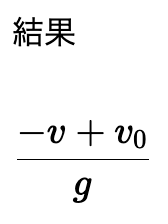
\includegraphics{work/pyodide_screenshot.png}
% \caption{実行結果} \label{Pyodide_result}
% \end{figure}

%%%%
\chapter{評価手法}

% 表の例
% \begin{table}[tb]
%  \begin{center}
%   \caption{Addistant 2の実行時間(秒)}
%   \label{tab:time}
%   \begin{tabular}{lr}
%    \hline
%                    & 時間 \\
%    \hline
%    X Window System & 15.0 \\
%    Addistant 1     &  3.0 \\
%    Addistant 2     &  2.0 \\
%    \hline
%   \end{tabular}
%  \end{center}
% \end{table}

% 表~\ref{tab:time}は...


%%%%
\chapter{まとめと課題} \label{conclusion}

\section{まとめ}
本研究では、学習者に物理系を定義させるシミュレータである \simname~(\simnamealt) を提案した。\simname では、物理法則から現象を数式で記述し、シミュレーションに変換するまでの工程も学習者が行う。これにより、従来は授業などで教わる必要があった現実の物理現象と物理法則の間の対応を学習者自らの経験を通して理解することができる。

\section{今後の課題}

\subsection{実装}

現在 \simname の機能のうち、
\begin{enumerate}
  \item 学習者の入力を Equation として解釈する
  \item 不正な次元の方程式になっていないかを確認する
  \item 数値計算するために数値を与える必要のある変数を推論する
\end{enumerate}
という部分が未実装である。それぞれについて方針を述べる。

\subsubsection*{学習者の入力を Equation として解釈する}
入力の解釈は、sympy.parsing.sympy\_parser の parse\_expr 関数を使うことで可能である。この関数では、文字列を SymPy のSymbol, Sum, Mul や Eq などに変換できる。実際に行う例を図~\ref{example_parse}に示す。一方、単にこれを用いるだけでは未定義の変数を使うことができてしまう。そのため、解釈された変数が定義されたものなのかを確認する必要がある。また、学習者がアンダースコアなどを入力する必要があったり、意図しない解釈をされる($v_Ax$ と $v_{Ax}$ など)可能性がある。Jupyter に表示されている変数をクリックすることでその変数を入力することができれば、このような誤りは防止でき、学習者の入力にかかる手間も減らすことができる。

\begin{figure}[htb]
  \centering
  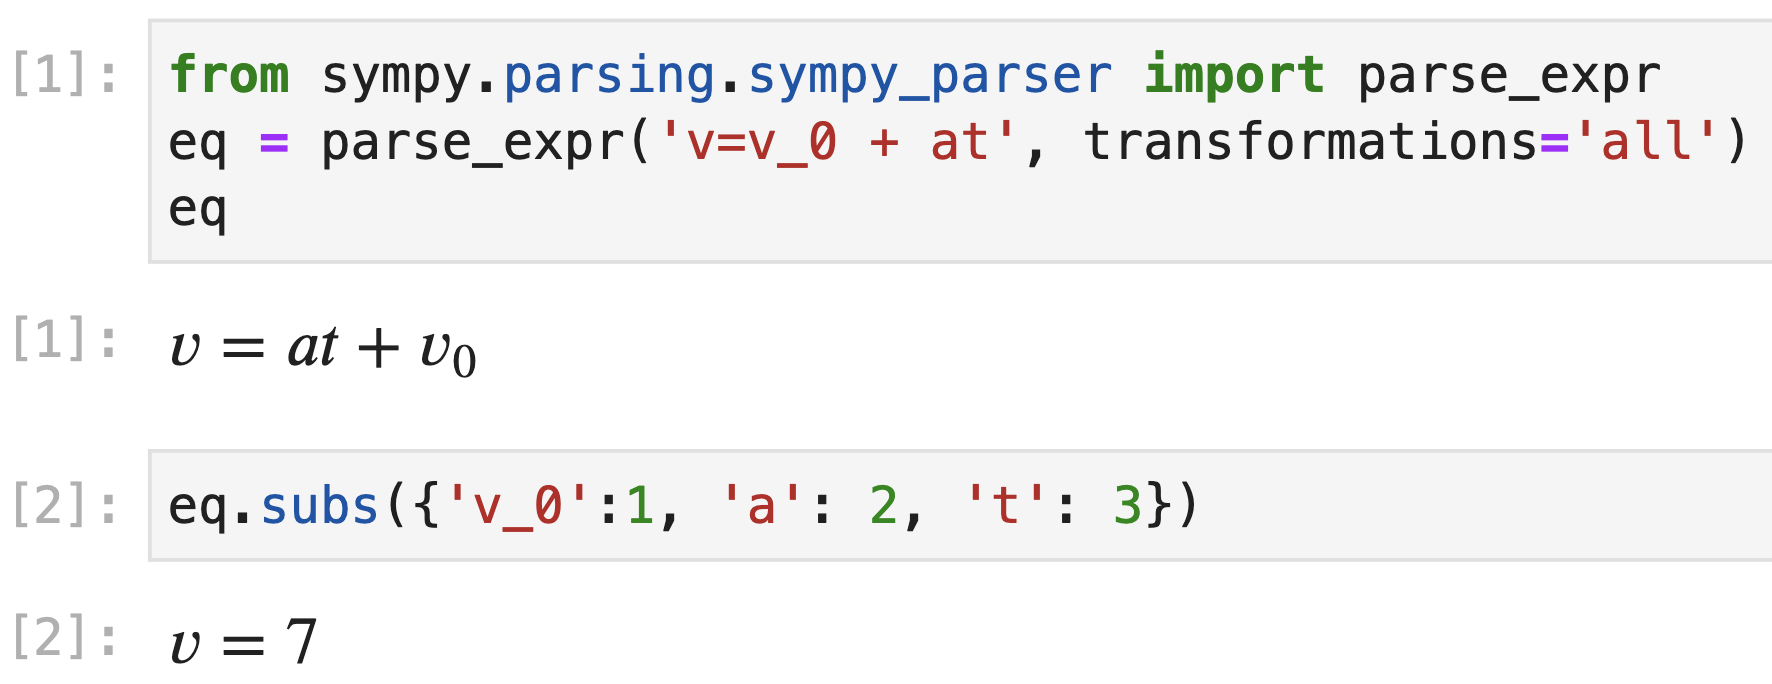
\includegraphics[width=0.9\linewidth]{work/example_parse.png}
  \caption{parse\_expr 関数で文字列をパースする例} \label{example_parse}
\end{figure}

\subsubsection*{不正な次元の方程式になっていないかを確認する}
現在の実装では、 $g + t~~\mathrm{([L/T^2] + [T])}$ のように次元が不正な方程式も定義できてしまう。SymPy の変数に次元の情報を付加し、異なる次元間の加減などを検出する必要がある。自動で追加される変数は生成する際に次元の情報を付加すればよいが、学習者が新たに追加する変数については次元を手動で指定する必要がある。L, M, T などの組み合わせを文字列で入力したものを解釈する、各次元の指数を数値で入力したものを解釈するなどの方法が考えられる。

\subsubsection*{数値計算するために数値を与える必要のある変数を推論する}
基本的には、学習者が定義した方程式に含まれる変数のうち物体に紐づいている位置・速度以外の変数の値を入力させれば良い。しかし、次のような場合も存在する。
\begin{align*}
x_A = X
X = v_0t
\end{align*}
ここで、$x_A$ は物体の $x$ 座標を表す変数で、$X$ と $v_0$ は学習者が定義した変数である。先述した方針では、$X$ と $v_0$ に値を入力する必要がある。しかし実際は $X$ か $v_0$ の一方にのみ値を入力すればよい。このような場合に対応する方法を考える必要がある。

\subsection{評価}

実装が完成したら、\simname の教育効果を評価する必要がある。高校生を、\simname を用いるグループ・PhET を用いるグループ・座学のグループに分け、pretest と posttest を行う。その結果を Hake~\cite{hake_1998}が導入した Normalized Gain を用いて比較することで、\simname の教育効果を測定できると考える。

また、\simname の利点は、現実の運動を確認できるだけでなく、現実の物理現象と物理法則の間の対応を学習者自らの経験を通して理解することができるという点である。そのため、各グループでディスカッションを行い、その内容からどれだけ現実の物理現象を正しく理解できているかを確認することも有効であると考える。

\clearpage
\section{発展のアイデア}

\simname を発展させるアイデアがいくつかあるので紹介する。

\subsection{他分野への対応}

現在の \simname の構成では、力学以外の分野に対応することが難しい。物体を追加した際の次元付き変数や観測ペインの可視化が力学を前提とした設計となっているためである。一方、高等学校で扱う物理には、音や光などの波動分野、回路や電場・磁場などの電磁気分野なども存在する。そのため、これらの分野にも対応できるようにしたい。

\subsection{方程式計算の強化}

現在、\simname 上に方程式を入力する際、その方程式の導出は学習者が行う必要がある。しかし、移項した際の符号の変え忘れや係数の間違いなど、\simname では検出できないミスが存在する。この作業を \simname でサポートしたい。

\subsubsection*{求解の自動化}
現在想定している \simname の実装では、物体に紐付けられている変数は他の変数で明示的に表されている必要がある。すなわち、$v_{Ax} = \sqrt{2gh}$ という表記は正しいが、$mgh = \dfrac{1}{2}mv_{Ax}^2$ という表記は受け付けない。このようなとき、SymPy を用いて $v_{Ax}$ を求めることができるため、計算ミスを防ぐことができる。一方、これを全て自動化してしまうと、学習者自身の方程式を変形する能力が成長しない。そのため、自動で求解するかどうかを切り替えられるようにする必要がある。

\subsubsection*{基本的な公式(運動方程式、力学的エネルギー保存則等)の提供}
物理学では、頻出する公式の数はある程度限られている。基本的な公式を提供し、各値に変数を割り当てるだけ方程式を定義することができるようにすれば、学習者の負担を大きく軽減することができる。これと先述した自動求解を組み合わせることで、適切な公式を選び適切に変数を割り当てるだけで物理系が作成できる。また、公式を解説付きで一覧にしたり、公式の検索機能をつけることで、公式を覚えきれてない初学者に対してもサポートができる。


%%%%%%%%%%%%%%%%%%%%%%%%%%%%%%%%%%%%%%%%%%%%%%%%%%%%%%%%%%%%%%%%%%%%%%

%
% 参考文献は直接書いてもいいが、bibtex を使うと便利
%  (1)このサンプルを platex にかける
%  (2)jbibtex thesis
%  (3)さらに platex にかける
%  (4)もう何回か platex にかける
%
% \bibliographystyle{csg-thesis}
\bibliographystyle{junsrt}
\bibliography{thesis}  %% thesis.bib というファイルを用意

%%%%%%%%%%%%%%%%%%%%%%%%%%%%%%%%%%%%%%%%%%%%%%%%%%%%%%%%%%%%%%%%%%%%%%

% 付録が必要ならつける
% \appendix
% \chapter{補足}

\section{モンキーハンティング} \label{モンキーハンティング}

以下のような形式の問題を総称してモンキーハンティングと呼ぶ。

\begin{quote}
小球を、位置 $(0, 0)$ から初速 $v_0$、 仰角 $\theta$ で発射したところ、位置 $(l, h)$ から自由落下してくる物体に衝突した。 $\tan \theta$ の満たすべき条件を求めよ。ただし、重力加速度の大きさを $g$ とする。
\end{quote}

\begin{figure}[htb]
\centering
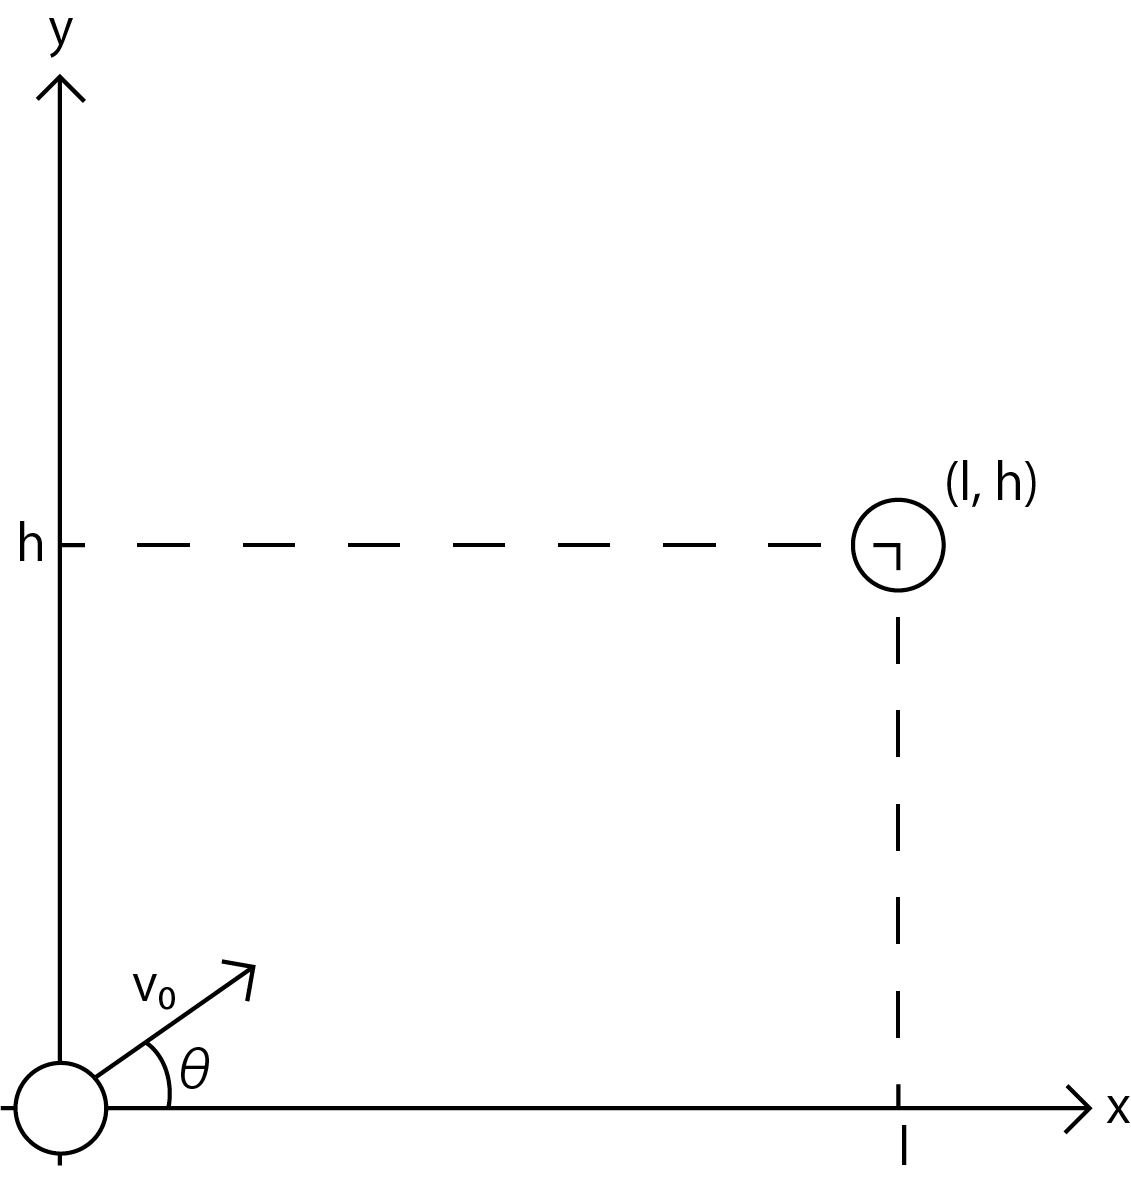
\includegraphics{work/monkey_hunting.png}
\end{figure}


\end{document}
